\chapter{Practical implementation}




During our research on stylization, we used Gratin \cite{vergne:hal-01254546} which a pipeline rendering software using \textit{OpenGL}. It permits to easily creates rendered images with \textit{GLSL} combining previous images as textures. As we said before every texture used from our contribution can be computed in parallel on GPU including the noises, the fractalization of the noises, the alpha blending and the splatting. Our method use only images as input so it can easily be integrated into every pipeline rendering. For example, if you have a pipeline rendering with \textit{path tracing} to compute the color of your scene you can use this rendered image as color input of our method without re-compute it.\newline

\begin{figure}[H]
    \begin{center}
    \fbox{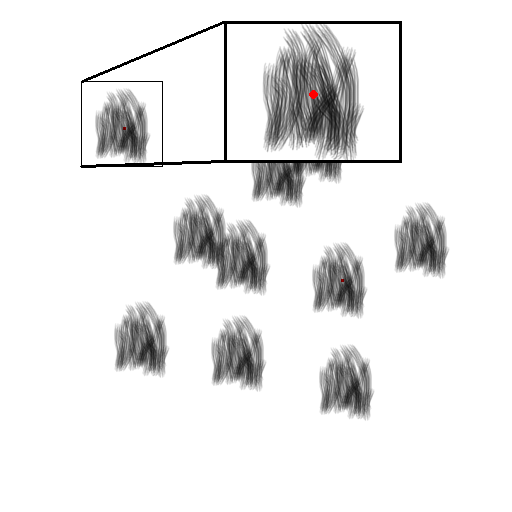
\includegraphics[width=60mm, height=60mm]{images/splatting/splatting4.png}}
    \end{center}
    \caption{Splatting principle: red dots are the anchor points and the splat is centered and anchored to this point.}
    \label{splatting_principle}
\end{figure}

For the splatting step, we draw on each pixel of the screen a square centered on the current pixel (see figure \ref{splatting_principle}). Every square is treated independently on the GPU before in the \textit{vertex shader} which manipulate the 4 vertices of the square which permits the resizing of the splat and permits the rotation of the splat. After this step of resizing and rotation, we pass in the \textit{fragment shader} which manipulate all pixels of splat. It is in this step that we will decide if we display the splat or not thanks to the procedural texture previously computed. \newline

\begin{figure}[H]
    \begin{center}
    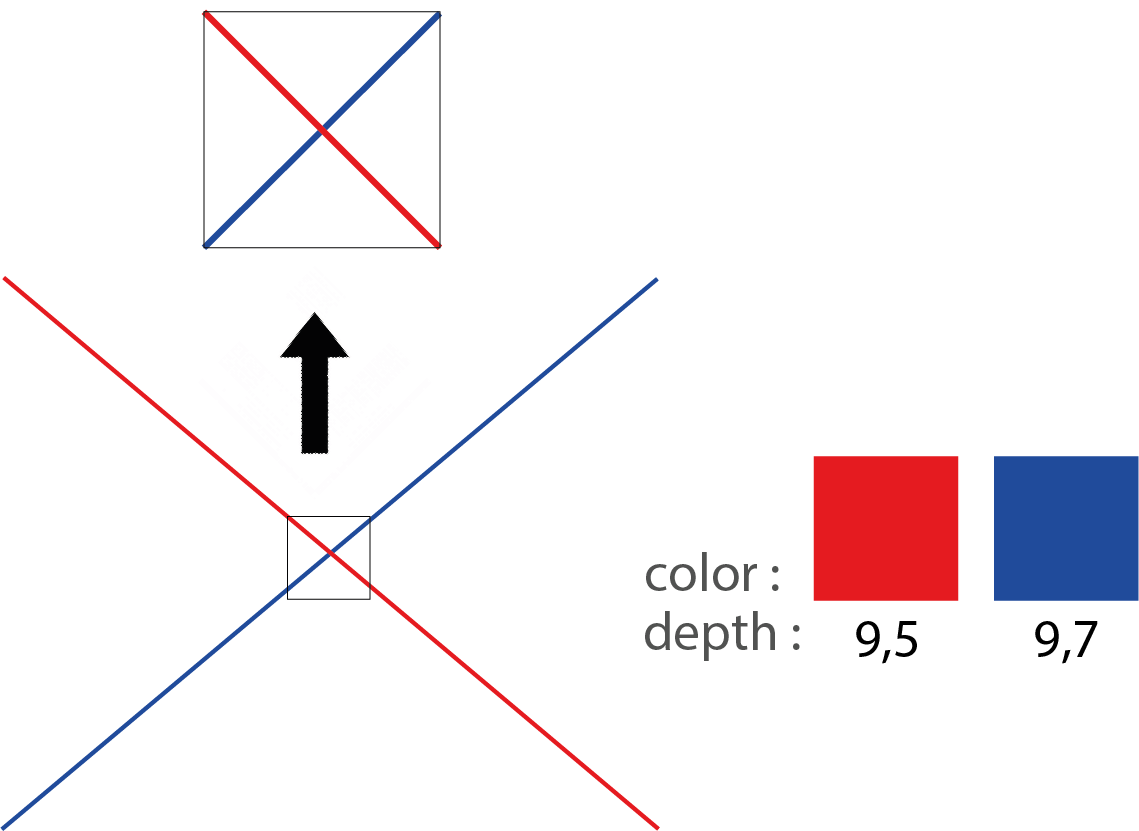
\includegraphics[scale=0.3]{images/splatting/order_independant_transparency.png}
    \end{center}
    \caption{Example of usage of the order independant transparency.}
    \label{order}
\end{figure}



In this \textit{fragment shader}, we prepare the technique of \textit{order-independent transparency} \cite{Munstermann} that consists of a structure that permit to know the order of the splats depending on the depth. We create in real time for each pixel of the screen a linked list on the GPU in order to sort the pixels contained in the splat. Thanks to this, we can apply a function of alpha blending that takes account the position of the splat, their color, their opacity. In our example in the figure \ref{splatting_principle}, we have some splats that cover others splats. How do we know which one is in front of the other if we treat them independently? For example, if there is a pixel where splat covers another one, we construct an array with 2 elements composed of color an depth so we can know which one is in front of the other one (see example in the figure \ref{order}). We apply the same technique but in our case we have a lot of splats that cover others and as depth to put in this array we use the depth corresponding to vertex of the stylized object where the splat is anchored (the red dots in the figure \ref{splatting_principle} correspond to a vertex of the 3d objects). \newline

After creating these array, we will in the last pass treat each pixel of the screen independently and (still on GPU) decide which color has to be displayed. In order to do this, we sort the array corresponding to the current pixel according to the depth. And finally, we apply our algorithm of alpha blending (the same as the mode "over" in Overcoat \cite{schmid_overcoat:_2011}): \newpage

\lstdefinestyle{customc}{
  belowcaptionskip=1\baselineskip,
  breaklines=true,
  frame=L,
  xleftmargin=\parindent,
  language=C,
  showstringspaces=false,
  basicstyle=\footnotesize\ttfamily,
  keywordstyle=\bfseries\color{green!40!black},
  commentstyle=\itshape\color{purple!40!black},
  identifierstyle=\color{blue},
  stringstyle=\color{orange},
}


\lstset{escapechar=@,style=customc}

\begin{lstlisting}
vec4 over(in vec4 c1,in vec4 c2) {
    float a = (c1.a+(1.-c1.a)*c2.a);
    return vec4((c1.rgb*c1.a + c2.rgb*(1.-c1.a)*c2.a)/a,a);
}

vec4 alpha_blending(vec4 colorArray[], int count, vec4 backgroundColor, float gammaBlend){
    // colorArray is the list of color sorted: colorArray[0] correspond to the farest
    // count corresponds to the number of splat that we will take account during the blending
    // backgroundColor is the color of the background our image
    // gammaBlend is a user parameter that will increase the transparency of the displayed color

    vec4 finalColor = vec4(0,0,0,0);

    for(int i=count-1; i>=0; i--) {
        vec4 currentColor = colorArray[i];
        finalColor = over(finalColor,vec4(currentColor.rgb,clamp(pow(currentColor.a,1./gammaBlend),0.,1.)));
    }

    return over(finalColor,backgroundColor);
}
\end{lstlisting}

After this algorithm, we have the color to display in the current pixel of the image/screen. With all these pixels, we have our final image.

% algo fractalization ????

% antialiasing
